%%%%%%%%%%%%%%%%%%%%%%%%%%%%%%%%%%%%%%%%%%%%%%%%%%%%%%%%%%%%%%%%%%%%%%%%%%%
%
% Fuzzy time domain
%
%%%%%%%%%%%%%%%%%%%%%%%%%%%%%%%%%%%%%%%%%%%%%%%%%%%%%%%%%%%%%%%%%%%%%%%%%%%
%INTRO
As explained in the introduction, humans handle temporal information using temporal notions like time intervals or time points~\cite{Dyreson1994}. While the used temporal notions may contain imperfections~\cite{Dev98},~\cite{Dubois:jucs_9_9:fuzziness_and_uncertainty_in},~\cite{nagypal2003},~\cite{Dubois89}, humans often gracefully deal with these, as their inherent interpretation capability accounts for a lot of them. This phenomenon has been studied a.o. in the field of artificial intelligence~\cite{Tre97},~\cite{5151} and language understanding~\cite{DeCaluwe:1997:FTI:285506.285516},~\cite{nagypal2003},~\cite{Dev98}. An information system, however, cannot appeal to a similar interpretation functionality. Thus, many proposals have been concerned with the combination of time and imperfections in the context of information systems~\cite{nagypal2003}. In this section, some main concepts and issues concerning this combination are presented.



\subsection{Types of Imperfections in Temporal Modelling}
Generally, in temporal modelling, a distinction is made between the following types of imperfections~\cite{nagypal2003}.



\begin{itemize}
	\item \emph{Uncertainty}: Temporal information or data may contain uncertainty. This means that the exact temporal value is (partially) unknown, however, generally some knowledge is present anyhow, possibly describing the value~\cite{Dubois:jucs_9_9:fuzziness_and_uncertainty_in},~\cite{nagypal2003},~\cite{Dubois89},~\cite{343607}. E.g., the temporal notion described in a sentence like `The Belfry of Bruges was finished on a day somewhere between 01/01/1201 A.D. and 31/12/1300 A.D.' contains uncertainty: it is known that the belfry of Bruges was finished on a single day and that this day lays somewhere between 01/01/1201 A.D. and 31/12/1300 A.D., but it is not known exactly which day it is.
	\item \emph{Vagueness}: Temporal information or data might contain inherent vagueness, as a precise instant or time interval may be intended, but the description of it is certainly vague~\cite{schockaert08},~\cite{nagypal2003},~\cite{Dev98}. E.g., the temporal notion described in a sentence like `It happened during summer.' contains vagueness, as even the boundaries of the mentioned temporal notion are not clearly expressed.
	\item \emph{Subjectivity or ambiguity}: Temporal notions might be subject to subjectivity or ambiguity. In certain cases, the temporal notion concerns a historical period like `late romanticism' or `the early middle ages' and thus contains subjectivity~\cite{nagypal2003}. In other cases, the interpretation of the temporal notion depends on extra factors. E.g., consider a person saying to another person `Let's meet each other at six.' The person hearing these words doesn't now if 6 a.m. or 6 p.m. is intended, though the person saying the words does.
\end{itemize}


As to the sources of the imperfections in temporal information, most proposals consider no specific source~\cite{5151},~\cite{schockaert08},~\cite{nagypal2003},~\cite{Dubois89},~\cite{343607},~\cite{ohlbach2004},~\cite{Virant199639}. Some proposals, however, deal with the imperfections specifically resulting from aspects of language~\cite{Dev98} and other proposals consider transitions between different granularities to be the source of imperfection in temporal information~\cite{Lin97}. Therefore, some proposals consider granularity as the base of the temporal model~\cite{Cru97}.





In an information system, temporal information is usually related to facts or events~\cite{Chountas2000}. In light of this, a classification of temporal information can be considered, in which the following types of temporal information may be found:


\begin{itemize}
\item \emph{Definite temporal information}:
Definite temporal information contains information describing a situation in which all time indications associated with some fact are absolute time indications. The temporal information is precisely known.

\item \emph{Indefinite temporal information}~\cite{Dey1996}:
Indefinite temporal information contains information describing a situation in which the time indication associated with some fact has not been fully defined. E.g., consider an event that in fact occured but it is not known exactly when.

\item \emph{Infinite temporal uncertain information}~\cite{Kabanza1990}:
Infinite temporal uncertain information contains information describing a situation in which an infinite number of time indications are associated with some fact. This is usually found in recurrent events like meetings. E.g., consider meetings that take place every Wednesday at noon. Some systems (usually with different information providers) may dispute the occurence and/or the duration of a fact.
\end{itemize}

\subsection{\label{subsec:representation}Representation of Imperfect Information}
As mentioned before, information systems may have to deal with time indications which contain vagueness. Even for some specific events or facts, the temporal indications may become imprecise. Therefore, a time point might be specified by means of a time interval of which the boundaries may not be precisely known. An example.

\begin{example}
Consider a speaker and a hearer. The speaker wants to make an appointment with the hearer. Now, consider the speaker saysing: \\
\begin{center}
\emph{`We will meet each other tomorrow around 10'}\\
\end{center}
The hearer will now usually instinctively agree that the appointment will be in e.g. the time interval between 9.55h and 10.05h.
\end{example}

The study of the semantics of `around' in temporal~\cite{Dev98} indications has shown that the size of the time interval associated with the imprecise specification of a time point depends on the distance with respect to the current time. E.g., consider now that the speaker is talking about something that happened \emph{`during last week'}, then the hearer would consider a time interval of more or less 10 days. 


Some proposals~\cite{knight1993},~\cite{Cru97},~\cite{nagypal2003},~\cite{Chountas2000} conclude that the best representation for incomplete temporal knowledge is therefore based on time intervals, even if they refer to a fact that happen at a time point. This means that, as Allen proposed in~\cite{Allen83}, the primitive units (the chronons) in a time domain, used in an information system should be intervals.

In order to represent and manage uncertain temporal information properly, several theoretical frameworks have been proposed:

\begin{itemize}
\item \emph{Probability theory}:
Probability theory~\cite{Dey1996},~\cite{Lakshmanan1997},~\cite{Haddawy1996} is usually employed when uncertainty concerning a time interval allows a probability to be associated to the time interval. The use of probability theory is very usual in logistics information systems. E.g., \emph{`The package will arrive at its destination on monday morning with a probability of 0.8'}.



\item \emph{Possibility theory}:
Using possibility theory~\cite{Dubois:Prade:1988:PossibilityTheory}, a possibility degree is associated to the temporal fact or event. Possibility theory is widely used to model uncertainty and vaguenes in time~\cite{Dubois:jucs_9_9:fuzziness_and_uncertainty_in},\cite{Dubois89},\cite{devos94},\cite{nagypal2003}. Several works~\cite{schockaert08},~\cite{ohlbach2004} present fuzzy versions of the temporal relations proposed by Allen~\cite{Allen83}. The aim of these works is generally to obtain a flexible way to compare uncertain, ill-known temporal intervals by means of temporal relationships.


\item \emph{Rough sets}:
Rough set theory~\cite{Pawlak1995} has been used to represent uncertainty in time intervals. The two dimensional representation of time intervals and the temporal relationships between them has been studied in~\cite{Qia09}.
\end{itemize}



\subsection{Imperfections in Temporal Relationships}
As the existence of temporal relationships allows to compare temporal notions, many approaches have been concerned with finding similar temporal relationships, able to support imperfections in the temporal information which is described by temporal notions or even by the temporal relationships themselves~\cite{ohlbach2004},~\cite{nagypal2003},~\cite{schockaert08},~\cite{Dubois:jucs_9_9:fuzziness_and_uncertainty_in}. These approaches are often based on Allen's operators~\cite{Allen83}. Example~\ref{ex:fuzzy-allen-relation} presents a short example concerning one of Allen's relationships.


\begin{example}
\label{ex:fuzzy-allen-relation}
Consider an event which takes place between time points $A$ and $B$. Thus, the event comprises time interval $[A,B]$ (this is visualized in part (1) of figure~\ref{fig:fuzzy-allen-relationship}). The classical Allen relationship `after' returns an interval $]B,\infty[$ as shown in part (2) of figure~\ref{fig:fuzzy-allen-relationship}. A fuzzified version of Allen's `after' operator is illustrated in part (3) of figure~\ref{fig:fuzzy-allen-relationship}. The comparison between two time intervals results in a possibility degree in the unit interval. The shape of the possibility distribution is shown in part (3) of figure~\ref{fig:fuzzy-allen-relationship}. Note that all the points strictly after the point $B$ results in a possibility degree of 1 whereas there is an area near the point $B$ in which the possibility degree runs smoothly between 0 and 1. 

Consider now the interval given by $[C,D]$, illustrated in part (4) of figure~\ref{fig:fuzzy-allen-relationship}. The user wants to know if $[C,D]$ is after $[A,B]$. The crisp version of the `after' operator would return \emph{`no'} as an answer. The fuzzy version for the same operator would return \emph{`yes, with a possibility of 0.5'}.


\begin{figure}
\centering
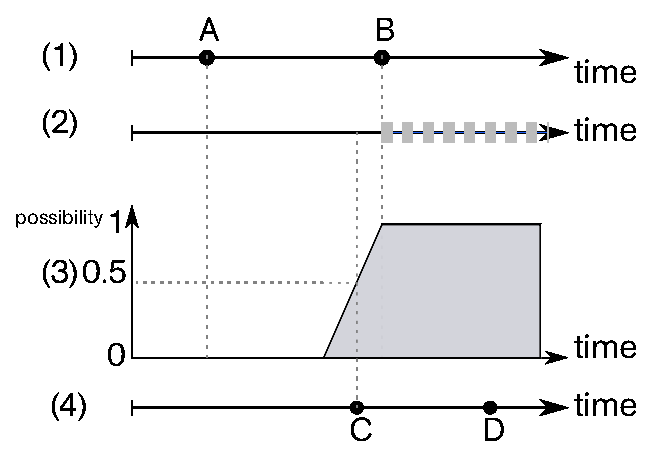
\includegraphics[scale=0.5]{graphs/fuzzyAllen.eps}
\caption{Example for the Allen relationship \emph{`after'}. (1) The event bounded within time points $A$ and $B$. (2) The crisp version of the \emph{`after'} operator. (3) A fuzzy version of the after operator. (4) Another event, bounded within time points $[C,D]$.}
\label{fig:fuzzy-allen-relationship}
\end{figure}
\end{example}




%%%%%%%%%%%%%%%%%%%%%%%%%%%%%%%%%%%%%%%%%%%%%%%%%%%%%%%%%%%%%%%%%%%%%%%%%%%
%
% End fuzzy time domain
%
%%%%%%%%%%%%%%%%%%%%%%%%%%%%%%%%%%%%%%%%%%%%%%%%%%%%%%%%%%%%%%%%%%%%%%%%%%%%%